\subsection{Shifumi}

    \begin{center}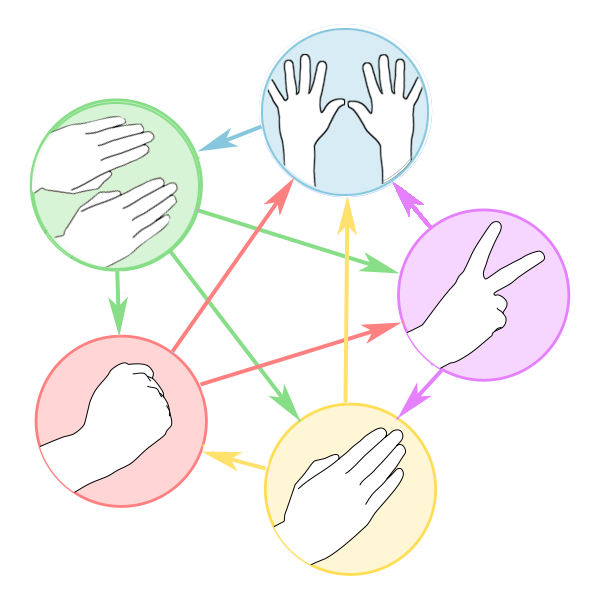
\includegraphics[width=6cm]{shifumi.png}\end{center}

    Une stratégie simple et efficace à laquelle on pourrait penser pour gagner
    au Shifumi serait de jouer de manière aléatoire.

    Et en effet, il s'avère que si les deux joueurs jouent de manière équiprobable,
    on a affaire à un équilibre de Nash~: aucun changement de stratégie de la part
    d'un joueur ne pourra lui permettre d'augmenter ses chances de gagner.
    %todo: expliquer plus Nash

    De plus, si un adversaire ne joue pas de manière aléatoire (ou augmente la
    probabilité de jouer un certain élément), alors on pourra prévoir ce qu'il
    va jouer et donc trouver une stratégie qui pourra le battre. Les humains
    étant très mauvais pour jouer de manière aléatoire, il est assez facile
    d'écrire une stratégie permettant de les battre.

  \subsubsection{Chaines de Markov}
    Une autre stratégie se base sur des chaines de Markov: en se basant sur les
    derniers éléments joués, elle regarde dans l'historique pour voir l'élément
    qui était joué le plus souvent par l'adversaire après les derniers coups
    joués.

    Cette stratégie s'avère vraiment efficace contre un joueur humain.
    Toutefois, elle est prévisible: si on sait qu'on a affaire à une telle
    stratégie, on peut jouer de manière à la battre.

    C'est pour cela qu'une stratégie aléatoire est la seule pouvant maximiser
    nos gains dans le pire des cas.

  \subsubsection{Variantes}
    Toutes les variantes du Shifumi qui consistent à rajouter des éléments
    pour obtenir un nombre d'éléments pair (par exemple
    pierre/papier/ciseaux/puits) vont créer un déséquilibre, car un élément
    sera moins efficace contre les autres.
    L'équilibre de Nash du jeu va
    alors consister à ne jamais jouer cet élément (et jouer aléatoirement parmi
    les autres).

    Si le nombre d'éléments est impair, alors le jeu pourra être équilibré,
    comme un Shifumi classique.

\subsection{Jeu de la somme magique}
  Ce jeu consiste à choisir, à tour de rôle, $n$ nombres entre 1 et $n^2$ afin
  que leur somme soit égale à $\frac{n(n^2+1)}{2}$.

  \subsubsection{Représentation sous forme de morpion}
Une représentation possible de ce jeu est le carré magique: les
joueurs doivent choisir, l'un après l'autre une case dans un carré
magique d'ordre $n$, leur but étant de contrôler une ligne, une colonne ou une
diagonale entière de ce carré magique; alors, les nombres qu'ils auront
choisis totaliseront le score voulu. De même, ce problème correspond exactement
au jeu du morpion, étendu à des grilles $n \times n$.

\begin{table}[h]
  \centering
  \begin{tabular}{|cccc|}
    \hline
    16 & 3  & 2  & 13 \\
    5  & 10 & 11 & 8  \\
    9  & 6  & 7  & 12 \\
    4  & 15 & 14 & 1  \\
    \hline
  \end{tabular}
  \caption{Un carré magique d'ordre 4 -- on remarque que les sommes des lignes,
    colonnes et diagonales sont biens égales à $\frac {4(4^2+1)} 2 = 34$}
\end{table}

Ainsi, une des stratégies possibles pour un joueur du jeu de la somme
magique est de construire un carré magique, et de représenter les
nombres choisis par l'adversaire par un rond dans la case
correspondante. Afin de choisir un nombre, il suffit d'appliquer la
stratégie de morpion de son choix sur le carré magique, et de
jouer le nombre correspondant.

Cependant, pour $n>3$, il n'y a pas un seul carré magique d'ordre $n$ (en
ignorant les réflexions et rotations). Cette méthode n'est donc exacte que dans
le cadre des morpions $3\times 3$. En effet, pour de plus grandes tailles les
deux joueurs pourraient jouer dans des carrés magiques différents. D'un point
de vu du morpion, on aura alors l'impression que l'adversaire joue n'importe
quoi, alors qu'il peut être en train de jouer correctement.

\paragraph{}
Le morpion étant un jeu où l'on essaie de minimiser la perte maximum,
on peut s'intéresser à l'algorithme du minimax, pour déterminer une
stratégie non perdante.

\subsubsection{Algorithme du minimax appliqué au jeu du morpion}
L'algorithme du minimax consiste à évaluer toutes les positions de jeu
atteignables depuis la position courante, sur une certaine profondeur
(autrement dit, un certain nombre de tours de jeu), et à jouer de
manière à atteindre la position la plus avantageuse, en supposant que
l'adversaire joue toujours le meilleur coup pour lui-même (ce coup
étant évalué avec notre propre fonction d'évaluation, qui n'est pas
forcément la même que celle de l'adversaire).

Par conséquent, afin d'implémenter l'algorithme du minimax, il faut
commencer par déterminer une fonction d'évaluation.

\paragraph{Fonction d'évaluation}
La fonction d'évaluation que nous avons choisie est très simple: une
ligne, colonne ou diagonale (que nous appelleront désormais simplement
``ligne'') complétée avec notre symbole (ce qui signifie qu'on a
gagné) vaut $+\infty$; si, au contraire, l'adversaire a complété une
ligne, alors cette ligne vaut $-\infty$. Une ligne contenant
uniquement notre symbole rapporte le nombre d'occurrences de notre
symbole dans cette ligne ; à l'inverse, une ligne contenant uniquement
le symbole de l'adversaire rapportera négativement le nombre.
Toutes les autres lignes ne rapportent aucun point.
Ainsi, l'évaluation d'une position de jeu est la somme des points
rapportés par chacune de ses lignes, colonnes et diagonales.

\paragraph{Minimax}
L'algorithme du minimax va construire (implicitement) l'arbre des coups
possibles à partir de la position courante.
L'évaluation d'un nœud de cet arbre sera:
\begin{itemize}
  \item si c'est à notre tour de jouer, le maximum de l'évaluation de nos fils;
  \item si c'est à l'adversaire de jouer, le minimum de l'évaluation
    de ses fils (i.e.\ on suppose que l'adversaire joue le meilleur
    coup à sa disposition, selon la fonction d'évaluation du joueur courant).
\end{itemize}

L'évaluation d'une feuille de l'arbre se fera par la fonction
d'évaluation définie précédemment.

Ainsi, l'algorithme se dirigera naturellement vers la position la plus
avantageuse pour lui.

\subsubsection{Élagage alpha-bêta}
L'élagage alpha-bêta permet de réduire le nombre de nœuds à parcourir durant
l'algorithme du minimax.

Cet algorithme arrête le parcours des fils d'un nœud quand il se rend
compte qu'il ne pourra pas faire mieux.

Dans l'exemple suivant, où les nœuds en bleus sont ceux où l'on doit prendre
le minimum, et ceux en gris le maximum:
\begin{multicols}{2}\begin{center}
  \begin{tikzpicture}[node distance=1.3cm,bend angle=45,auto]
    \node[draw, rectangle, gray] (U) {U};
    \node[draw, circle, blue] (5) [below left=of U] {5};
    \node[draw, circle, blue] (V) [below right=of U] {V};
    \node[draw, rectangle, gray] (4) [below left=of V] {4};
    \node (dots) [below right=of V] {\ldots};

    \path (U) edge node {} (5);
    \path (U) edge node {} (V);
    \path (V) edge node {} (4);
    \path (V) edge node {} (dots);
  \end{tikzpicture}

  Coupure Alpha

  \begin{tikzpicture}[node distance=1.3cm,bend angle=45,auto]
    \node[draw, circle, blue] (U) {U};
    \node[draw, rectangle, gray] (5) [below left=of U] {5};
    \node[draw, rectangle, gray] (V) [below right=of U] {V};
    \node[draw, circle, blue] (4) [below left=of V] {4};
    \node (dots) [below right=of V] {\ldots};

    \path (U) edge node {} (5);
    \path (U) edge node {} (V);
    \path (V) edge node {} (4);
    \path (V) edge node {} (dots);
  \end{tikzpicture}

  Coupure Béta
\end{center}\end{multicols}

On se rend bien compte qu'on n'a pas besoin de parcourir les nœuds suivant,
car on prend le maximum des minimums, ou l'inverse.

Par exemple, pour la coupure alpha: si on trouve des fils de $V$ plus petit
que $4$, on va prendre le maximum, donc c'est $4$ qui sera utilisé, et si on
trouve plus grand ou égal à $5$, on devra prendre le minimum au niveau de $V$,
donc on prendra $5$ dans tous les cas.

Au final, cette amélioration permet de gagner un temps considérable pour
obtenir le même résultat.


\subsection{Duopôles}
  Les jeux précédents sont des jeux non coopératifs à somme nulle (on peut soit
  gagner, soit perdre).

  Il peut aussi être intéressant de voir les jeux à somme non nulle, c'est à
  dire qu'il n'y a pas forcément un gagnant ($1$ point) et un perdant ($-1$
  point), mais il est possible de faire des situations plus ou moins
  gagnant-gagnant, voire même perdant-perdant.

  Le duopôle de Cournot est un bon exemple de ce genre de jeu: il met en jeu
  deux entreprises qui produisent des biens sur le même marché. Elles se font
  donc concurrence, mais plus le marché est inondé de produits, plus leur marge
  est faible (elles peuvent même faire des pertes!).

  \subsubsection{Modélisation}
    On modélise le cout de production unitaire par une constante $\gamma$,
    et le prix de vente unitaire est une fonction affine décroissante de la
    production totale $x+y$ (où $x$ est la production d'une entreprise, et $y$
    celle de l'autre): $p(x, y) = \alpha - \beta\times (x + y)$. Il est bien
    évidemment commun aux deux entreprises.

    Les gains des entreprises sont donc respectivement:
      \[\begin{array}{c}
        g_1(x, y) = x\times (p(x, y)-c(x)) = x(\alpha+\gamma-\beta(x+y)) \\
        g_2(x, y) = y\times (p(x, y)-c(y)) = y(\alpha+\gamma-\beta(x+y))
      \end{array}\]

    Par la suite, nous noterons $a=\alpha+\sigma$.

  \subsubsection{Stratégies possibles}
    \paragraph{Coopération} Il est possible de coopérer complètement avec
      l'adversaire, en partant du principe que s'il produit autant que nous,
      on maximisera le gain commun de chaque entreprise.
      Cette stratégie permet de très bons gains avec toute autre stratégie qui
      coopère, mais elle se fera souvent écraser par des stratégies qui vont
      «~profiter d'elle~».

      Pour coopérer il suffit de maximiser $g_1(x, y)+g_2(x, y)$ par rapport à
      $x+y$ soit
        \[g_1(x, y) + g_2(x, y) = 2(x+y)(a - \beta(x+y))\]

      Le maximum est donc atteint en $x+y=\frac a {2\beta}$.

      Pour que chaque entreprise ait le même gain, on a $g_1(x, y) = g_2(x, y)$.
      Elles doivent donc produire $x=y=\frac a {4\beta}$.

    \paragraph{Stackelberg}
      % on profite de l'autre, toussa
      TODO

    \paragraph{Œil pour œil, dent pour dent}
      Le principe de cette stratégie est d'être coopérative tant que
      l'adversaire l'est, et de devenir plus agressive quand il ne l'est plus:
      à chaque fois que l'autre joueur n'est pas coopératif, on joue comme le
      ferait la stratégie Stackelberg.

      Une variante de cette stratégie consiste à le pénaliser de plus en plus:
      la première fois on le pénalise une fois, puis deux, puis trois, etc.

      Ces deux stratégies sont efficaces à la fois quand l'autre joueur est
      coopératif (on est alors coopératif) et contre un joueur non-coopératif
      (on devient alors agressif).
